\section{Verkehrsanalyse}
Der nächste Schritt nach der Auswahl der geographischen Parameter ist die Verkehrsanalyse. In diesem Kapitel sollen im Sinne einer Machbarkeitsstudie Möglichkeiten aufgezeigt werden die Verkehrsdaten zu visualisieren und zu analysieren. Danach werden sie auf eine repräsentative Zahl, also einen \grq Stauindex\grq  reduziert.\\
Das Ziel der Auswertung der Verkehrsdaten ist es die Verkehrssituation in Städten über einen längeren Zeitraum bewerten zu können und eine Vergleichbarkeit zwischen Städten herzustellen. Ein Stauindex kann hier einen einfachen Überblick über die Daten gewährleisten.\\ Zu verkehrlich besonders interessanten oder auffälligen Zeiten bietet es sich an auf die detaillierteren Daten zurückzugreifen um einen besseren Überblick über die Situation zu gewinnen.

\subsection{Aufbau der Verkehrsdaten}
Die Verkehrsdaten werden von Bing Maps durch Einfärben der Straßen in 4 verschiedenen Farben für die verschiedenen Verkehrszustände bereitgestellt. Es gibt die Zustände kein Verkehr (grün), wenig Verkehr (gelb), mittlerer Verkehr (orange) und dichter Verkehr (rot). Abbildung~\ref{fig:farben_einfuehrung} zeigt beispielhaft einen Ausschnitt der Verkehrssituation in Karlsruhe aus Bing Maps. Insbesondere fällt auf, dass Bing Maps für zahlreiche verkehrsrelevante Straßen in Karlsruhe keine Verkehrsinformationen enthält.\\
\begin{figure}
  \centering
    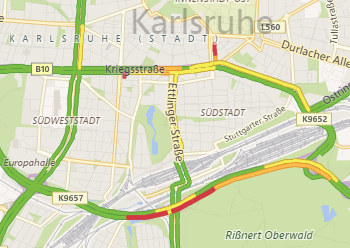
\includegraphics[width=0.7\textwidth]{images/verkehr_einfuehrung.png}
    \caption{Beispielhafte Verkehrsdaten aus Bing Maps. Die Daten repräsentieren die  Verkehrszustände: kein Verkehr (grün), wenig Verkehr (gelb), mittlerer Verkehr (orange) und dichter Verkehr (rot)}
    \label{fig:farben_einfuehrung}
\end{figure}

Die angegebenen Farben sind dabei nur bedingt proportional zur Verkehrsstärke und eher als Beeinflussung der Verkehrssituation, statt als Menge der Fahrzeuge pro Zeiteinheit zu sehen. Abbildung~\ref{fig:uebersicht_verkehrszustaende} zeigt Beispielhaft die Aufnahmen von Verkehrskameras mit den zu der Zeit in Bing Maps angezeigten Verkehrszuständen.\\  
\begin{figure}
\begin{tabular}{@{}cc@{}}
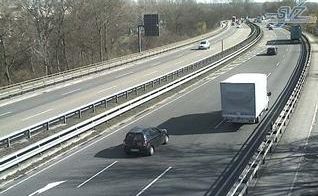
\includegraphics[width = 0.48\textwidth]{images/no_traffic.png} &
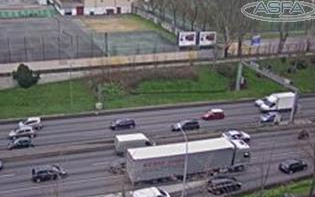
\includegraphics[width = 0.48\textwidth]{images/low_traffic.png} \\ 
\textbf{kein Verkehr}  & \textbf{leichter Verkehr}   \\
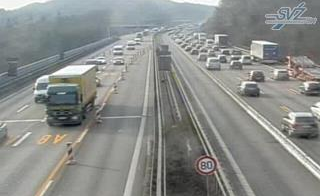
\includegraphics[width = 0.48\textwidth]{images/medium_traffic.png} & 
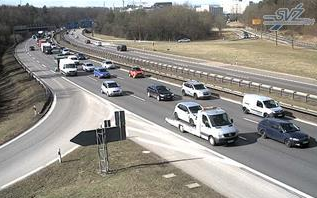
\includegraphics[width = 0.48\textwidth]{images/heavy_traffic.png} \\
\textbf{mittlerer Verkehr} & \textbf{dichter Verkehr}\\
\end{tabular}
\caption{Bilder von Verkehrskameras zu den Verkehrszustände kein Verkehr, leichter verkehr, mittlerer Verkehr und dichter Verkehr aus Bing Maps}
\label{fig:uebersicht_verkehrszustaende}
\end{figure}

Mit der in Kapitel~\ref{chapter:christof} beschriebenen Methode lassen sich die Verkehrsinformationen auslesen und die Anteile der jeweiligen Verkehrszustände an allen Pixeln mit Verkehrsinformation ermitteln.
Eine Möglichkeit die Anteile der Verkehrszustände graphisch anschaulich darzustellen ist als gestapelter Graph.
Abbildung~\ref{fig:stacked_stuttgart} zeigt die Anteile von leichtem, mittlerem, und dichtem verkehr in Stuttgart am Dienstag, dem 06.02.2017. Die Form der summierten Anteile entspricht sehr gut der aus dem Verkehrswesen bekannten Tagesganglinie. 
\begin{figure}
  \centering
    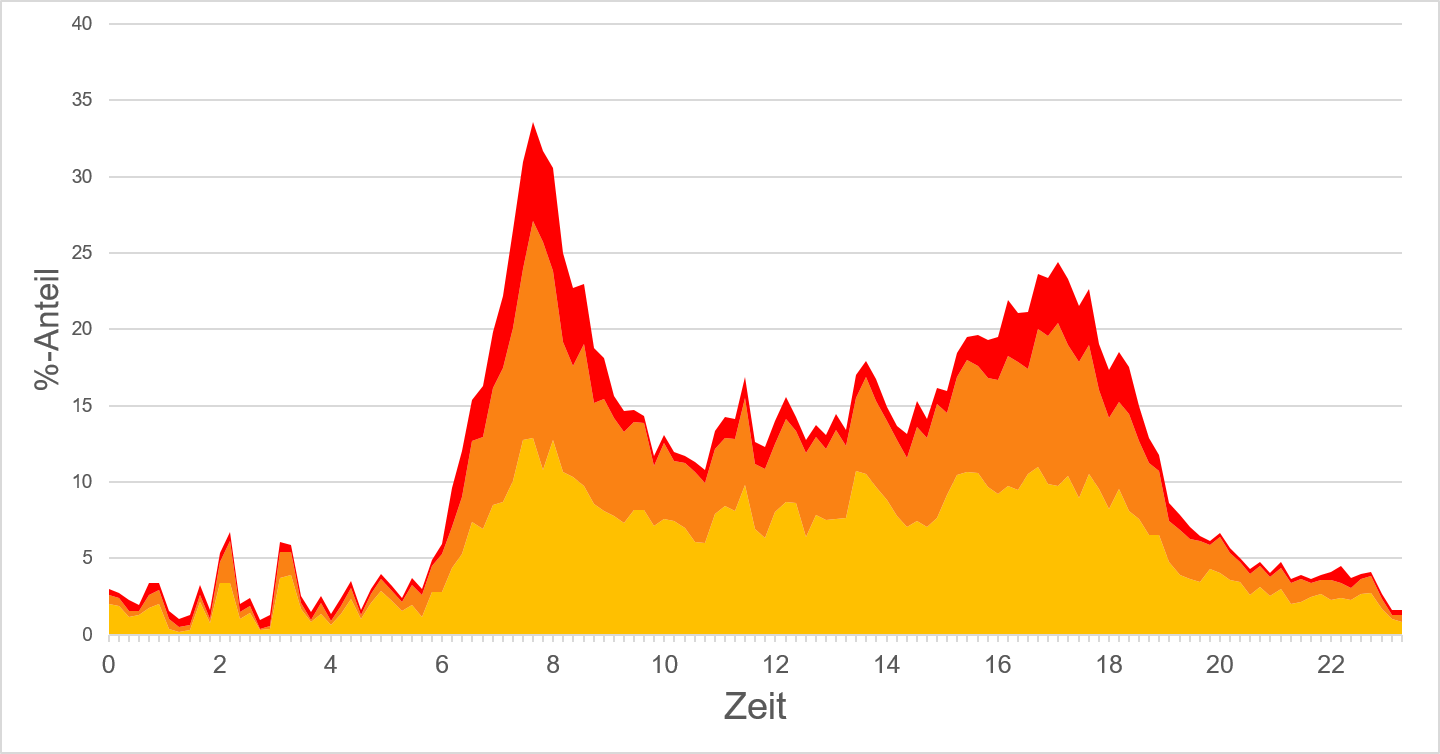
\includegraphics[width=1.0\textwidth]{images/stacked_stuttgart.png}
    \caption{Prozentualer Anteil der Verkehrszustände wenig Verkehr (gelb), mittlerer Verkehr (orange) und dichter Verkehr (rot) an allen Pixel auf dem Kartenausschnitt, die mit Verkehrsinformationen belegt sind.}
    \label{fig:stacked_stuttgart}
\end{figure}

\subsection{Stauindex}

Ausgehend von den Assoziationen mit dem Wort Stauindex lassen sich folgende Anforderungen ableiten:
\begin{itemize}
\item Der Stauindex soll die verschiedenen Verkehrszustände entsprechend ihrer Beeinträchtigung der Verkehrsteilnehmer unterschiedlich stark gewichten.
\item Er soll außerdem Verkehrszuständen mit stärkerer Beeinträchtigung der Verkehrsteilnehmer einen höheren Index zuweisen.
\item Um eine Vergleichbarkeit zwischen Städten  herstellen zu können, soll der Index sich auf die mit Verkehrsinformationen belegte Fläche beziehen. Andernfalls würde der ausgewählte Kartenausschnitt in Kombination mit der Struktur der Stadt eine sehr große Rolle spielen. 
\end{itemize}
Diese Voraussetzungen lassen sich mit folgender Gleichung abbilden:

\begin{equation}\label{eq:1}
\frac{\beta_l\cdot p_{leicht}+\beta_m\cdot p_{mittel}+\beta_d\cdot p_{dicht}}{P_{mit Info}}
\end{equation}
\begin{itemize}
\item $\beta_l$: Gewichtungsfaktor für leichten Verkehr
\item $p_{leicht}$: Anteil an leichtem Verkehr
\item $\beta_m$: Gewichtungsfaktor für mittleren Verkehr
\item $p_{mittel}$: Anteil an mittlerem Verkehr
\item $\beta_d$: Gewichtungsfaktor für dichten Verkehr
\item $p_{dicht}$: Anteil an dichtem Verkehr
\item $p_{mit Info}$: Anteil der mit Verkehrsinformationen belegten Pixeln
\end{itemize}

Bei der Abbildung der Verkehrssituation auf einen Stauindex und der Vergleichbarkeit zwischen Städten treten mehrere Probleme auf. Zum einen wird die Verkehrssituation in verschiedenen Städten aufgrund der unterschiedlichen Datenverfügbarkeit von Bing Maps unterschiedlich dargestellt. Große Städte wie Berlin verfügen oft über sehr umfangreiche Verkehrsinformationen. In kleinen und mittelgroßen Städten sind i.d.R. nur Verkehrsinformationen für die größten Straßen verfügbar, während andere verkehrlich relevante Straßen über keine Informationen verfügen.\\ Der Mangel an Informationen deutet in erster Linie auf wenig Verkehrsteilnehmer und somit eine gute Verkehrssituation hin. Jedoch können die Gründe hierfür auch in den von Bing Maps verwendeten Algorithmen oder einem geringen Smartphonebesitz liegen. Dies führt zu einer schlechteren Darstellung der Verkehrssituation in kleinen und mittelgroßen Städten, da der guten Verkehrssituation auf verkehrlich relevanten Straßen nicht Rechnung getragen wird.\\  
Eine Möglichkeit dieses Problem zu beheben besteht darin, die aus Google Maps ermittelte gesamte Straßenfläche einer Stadt mit einem Gewichtungsfaktor einzubeziehen. Dabei bleibt jedoch die Frage offen, welcher Anteil der Straßen einer Stadt als verkehrlich relevant anzusehen ist.\\
Ein weiteres Problem besteht zu Schwachlastzeiten, wenn besondere Verkehrsbeeinträchtigungen eintreten. Zu diesen Zeiten sind aufgrund der geringen Anzahl an Verkehrsteilnehmern weniger Straßen mit Verkehrsinformationen belegt. Dieser Zustand ist in Abbildung~\ref{fig:stauindex_problem} beispielhaft dargestellt. 

\begin{figure}
  \centering
    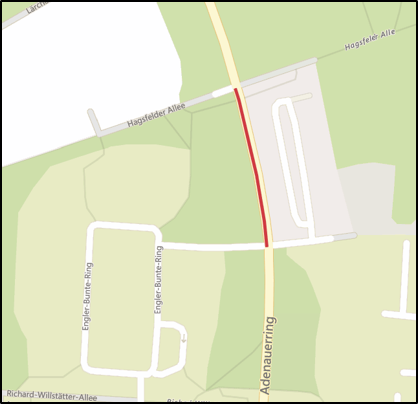
\includegraphics[width=0.5\textwidth]{images/stauindex_problem.png}
    \caption{Problematische Situation bei Berechnung des Stauindex ohne Betrachtung des gesamten Straßenfläche. Diese Situation würde aufgrund der hohen Anzahl an Pixeln mit dichter Verkehrssituation bei insgesamt geringer Verfügbarkeit von Verkehrsinformationen zu einem sehr hohen Stauindex führen.}
    \label{fig:stauindex_problem}
\end{figure}

Ist nun ein Teil der Straßen z.B. durch eine Baustelle oder einen Unfall mit einem mittleren oder dichten Verkehrszustand belegt, führt dies mit Gleichung~\ref{eq:1} zu einem besondere hohen Stauindex. In diesem Fall kann ebenfalls auf die gesamte Straßenfläche zurückgegriffen werden, um den Stauindex zu reduzieren.
Der Stauindex kann auf folgende Weise modifiziert werden, im die gesamte Straßenfläche zu beachten.

\begin{equation}\label{eq:2}
\frac{\beta_l\cdot p_{leicht}+\beta_m\cdot p_{mittel}+\beta_d\cdot p_{dicht}}{P_{mit Info} + \beta_o\cdot P_{ohne Info}}
\end{equation}

\begin{itemize}
\item $\beta_o$: Gewichtungsfaktor für Straßen ohne Verkehrsinformation
\item $p_{ohne Info}$: Anteil der Straßen ohne Verkehrsinformation
\end{itemize}

Die Ergebnisse von Gleichung~\ref{eq:2} sind am Beispiel eines Dienstags in Stuttgart in Abbildung~\ref{fig:stauindex_stuttgart} dargestellt. Hier zeigt sich ebenfalls die bekannte Form der Tagesganglinie. Die Höhe der Morgen- und Abendspitze hängt aufgrund der hohen Anteile von mittlererm und dichtem verkehr stark von der Wahl der Gewichtungsfaktoren ab.\\

\begin{figure}
  \centering
    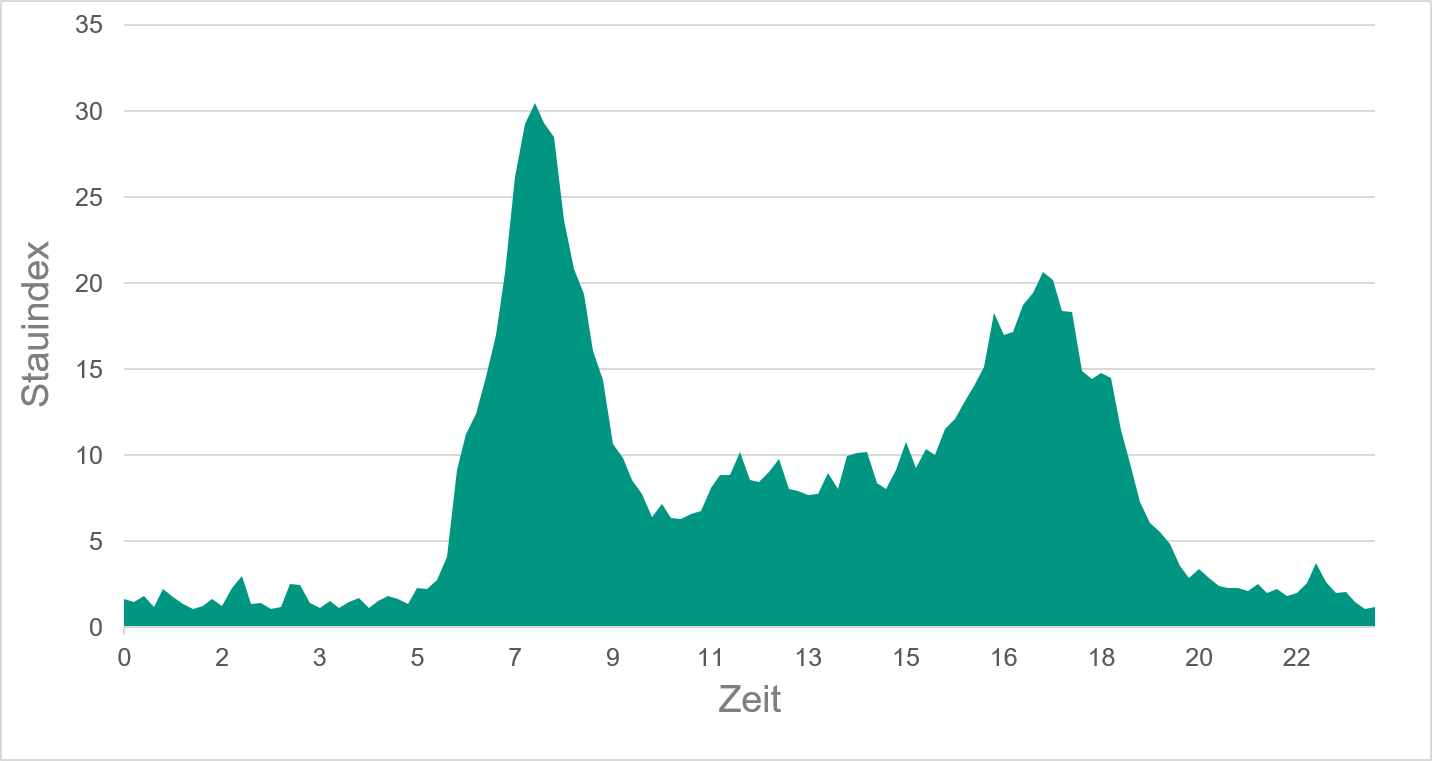
\includegraphics[width=1.0\textwidth]{images/stauindex.png}
    \caption{Stauindex der Stadt Stuttgart während eines Dienstag über einen Zeitraum von 24 Stunden in 10-Minuten-Intervallen aufgenommen.}
    \label{fig:stauindex_stuttgart}
\end{figure}

Der Stauindex bezieht sich bislang nur auf einen Zeitpunkt. Im Sinne eines übersichtlichen Index soll jedoch der Gesamtverkehrssituation über einen längeren Zeitraum ein Index zugeordnet werden. Hierfür bestehen mehrere Möglichkeiten den Index zeitlich zu mitteln. Eine Möglichkeit besteht darin, den arithmetischen Mittelwert über den gesamten Zeitraum zu bilden.\\ Dies hat den Vorteil, dass besondere Verkehrszustände, welche i.d.R nicht den ganzen Tag über anhalten, weniger stark gewichtet werden. Somit ist ein repräsentatives Ergebnis bereits bei geringer Datenverfügbarkeit möglich.
Nachteil dieser Methode ist, dass die Verkehrssituation des ganzen Tages berücksichtigt wird, wobei aber i.d.R. nur die morgendliche und abendliche Hauptverkehrszeit zu wesentlichen Beeinträchtigungen führt.\\ Qualitative Untersuchungen der gesammelten Daten zeigen, dass die Zustände mittlerer- und dichter Verkehr nur während der Hauptverkehrszeit in wesentlichen Mengen auftreten und auf einer Basis des Zustands leichter Verkehr aufsetzen, der während des Tages relativ konstant bleibt und nur in den Schwachlastzeiten abfällt (siehe Abbildung~\ref{fig:stacked_stuttgart}). Diese Basis an leichtem Verkehr kann bei entsprechender Wahl der Gewichtungsfaktoren den Stauindex stark negativ beeinflussen, was dem Prinzip eines Stauindex widersprechen würde. Dieses Problem tritt insbesondere in großen Städten mit hoher Verfügbarkeit an Verkehrsdaten auf.\\ Alternativ zum arithmetischen Mittelwert des Tages ist es auch möglich einen Hauptverkehrszeit-Stauindex zu bilden. Hierfür wird das arithmetische Mittel über eine festzulegende Anzahl an Maximalwerten pro Tag gebildet. Dies löst das diskutierte Problem des des leichten Verkehrs und es wird die Verkehrssituation einer Stadt zur verkehrlich relevante Zeit betrachtet. Die Anfälligkeit gegenüber besonderen Verkehrsereignissen, wie z.B. Staus, steigt jedoch stark an und es ist somit eine wesentlich größere Datenbasis erforderlich. \\


Tabelle~\ref{fig:index_tabelle} zeigt das arithmetische Mittel des ganzen Tages, das Maximum und das Minimum zwischen 8 und 20 Uhr des Stauindex für ausgewählte Städte. Der Index wurde mit Gleichung~\ref{eq:2} berechnet, als Datenbasis wurde ein Zeitraum von 24 Stunden während eines Dienstag verwendet. Die Ergebnisse sind somit nicht repräsentativ für die jeweiligen Städte, zeigen aber aufgrund der Ähnlichkeit, dass es mit weiteren Untersuchungen der Gewichtungsfaktoren und der Kartenausschnitte und einer wesentlich größeren Datenbasis möglich sein könnte eine Vergleichbarkeit der Städte herzustellen.





\begin{figure}
  \centering
    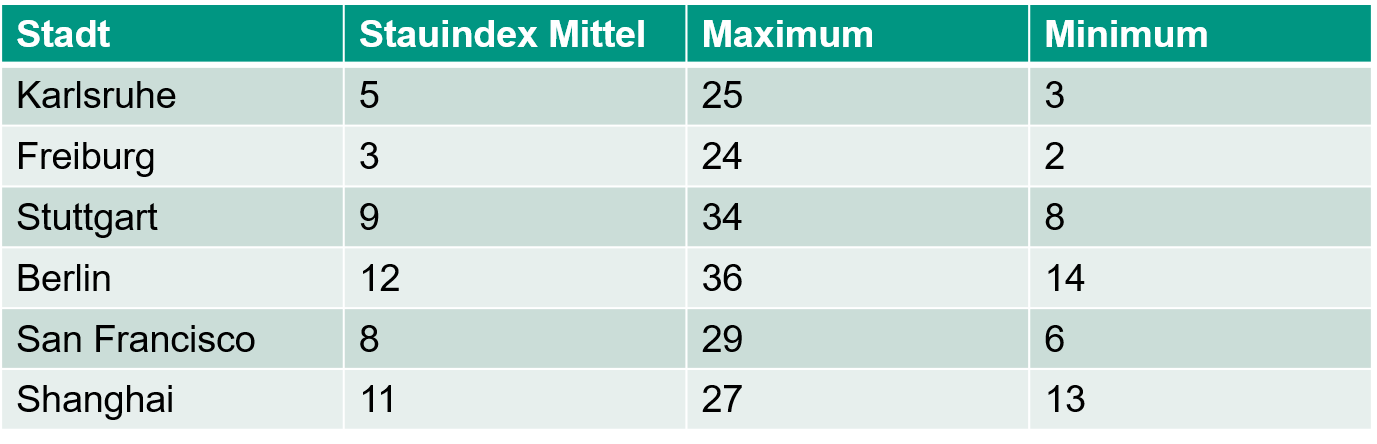
\includegraphics[width=1.0\textwidth]{images/index_tabelle.png}
    \caption{Arithmetisches Mittel des ganzen Tages, Maximum und Minimum zwischen 8 und 20 Uhr des Stauindex für ausgewählte Städte auf Datenbasis eines Dienstages.}
    \label{fig:index_tabelle}
\end{figure}